To develop the e-learning platform 3 main modules were identified: UI, Services and Execution Environments.
\\
The UI module is the presentation layer, with which the final user will interact. This interface will be developed with React, a JavaScript library for building user interfaces, as a single page application.
\\
	\begin{wrapfigure}{l}{0.7\textwidth}
  		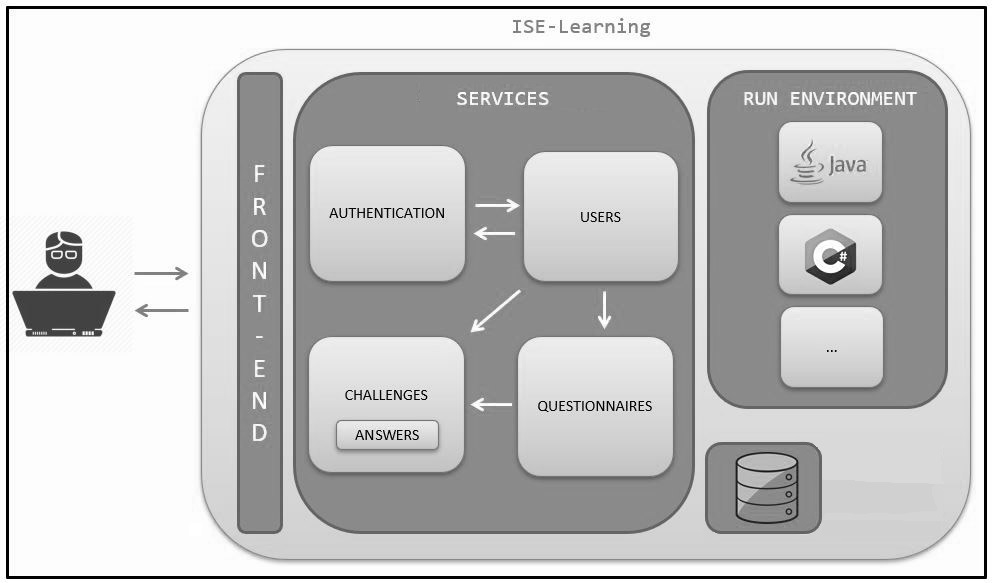
\includegraphics[scale=0.6]{./imgs/arquitectura.JPG}
  		\caption{Architecture}
  		\label{fig:architecture}
	\end{wrapfigure} 
The Services module will provide a REST API which is the core of the platform, this module will be developed using a microservice architecture. This REST API can be used standalone or with the UI module. In this project the REST API will be used to support the UI module. This module will be developed with the following technological stack: Kotlin; Gradle; Spring; Docker; Postgres; Swagger; Cloud based hosting solution.
\\
Kotlin is the programming language which will be used to develop the microservices, Gradle will be used for dependency management, Spring will be used as a support framework for dependency injection and REST application development.
\\
Docker will be used to build and run containers for each microservice and the database. Postgress will be used as the SQL client to enable data persistence across the platform. Swagger will be used to document the REST API and a cloud based solution will be used to host the platform, on a later date a comparative analysis will be done to find the right solution for this project with the major cloud providers (GCP, Azure, AWS).
\\
 
The Execution Environment module will be responsible for executing code provided by an external source. This module will support several runtime environments, where each application will be developed and hosted on a separate container.
\\[2ex]
Some risk were identified during the project analysis: scalability, requires extensive load tests with the solution deployed on cloud environment; lack of diverse userbase for testing, complex solutions required thorough testing to minimize bugs; group members are currently working and studying at same time; the learning process required for new tools has inherent uncertainty; estimates may not meet proposed values.
\\
The major constraint of this project's execution is time management. Taking this into account several strategies were devised as contingency plans if need be: scope reduction, removing questionnaire functionality; group members taking personal vacation days; drop one of the other courses.